% !TEX TS-program = pdflatex
% !TEX encoding = UTF-8 Unicode


\documentclass[11pt]{article} % use larger type; default would be 10pt

\usepackage[utf8]{inputenc} % set input encoding (not needed with XeLaTeX)
\usepackage[portuges]{babel}


%%% PAGE DIMENSIONS
\usepackage{a4}

\usepackage{graphicx} % support the \includegraphics command and options
\graphicspath{ {./UI/}{./VPP/}{./UCASES/}}
%%% PACKAGES
\usepackage{booktabs} % for much better looking tables
\usepackage{array} % for better arrays (eg matrices) in maths
\usepackage{paralist} % very flexible & customisable lists (eg. enumerate/itemize, etc.)
\usepackage{verbatim} % adds environment for commenting out blocks of text & for better verbatim
\usepackage{subfig} % make it possible to include more than one captioned figure/table in a single float
% These packages are all incorporated in the memoir class to one degree or another...

\usepackage{xcolor}


%%% HEADERS & FOOTERS
\usepackage{fancyhdr} % This should be set AFTER setting up the page geometry
\pagestyle{fancy} % options: empty , plain , fancy
\renewcommand{\headrulewidth}{0pt} % customise the layout...
\lhead{}\chead{}\rhead{}
\lfoot{}\cfoot{\thepage}\rfoot{}

%%% SECTION TITLE APPEARANCE
\usepackage{sectsty}
\allsectionsfont{\sffamily\mdseries\upshape} % (See the fntguide.pdf for font help)
% (This matches ConTeXt defaults)

%%% ToC (table of contents) APPEARANCE
\usepackage[nottoc,notlof,notlot]{tocbibind} % Put the bibliography in the ToC
\usepackage[titles,subfigure]{tocloft} % Alter the style of the Table of Contents
\renewcommand{\cftsecfont}{\rmfamily\mdseries\upshape}
\renewcommand{\cftsecpagefont}{\rmfamily\mdseries\upshape} % No bold!

\title{Projeto de DSS \\ \large ConfiguraFácil - Relatório}
\date{2018/19}

\begin{document}
\maketitle

\begin{table}[!htbp]
\centering
\begin{tabular}{cc}
 Diogo Sobral (a82523) &  Henrique Pereira (a80261) \\
 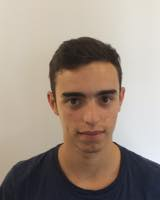
\includegraphics[height=0.8in]{Diogo} &  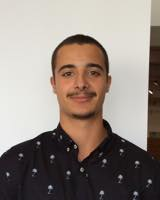
\includegraphics[height=0.8in]{Henrique} \\
	& \\
 Pedro Moreira (a82364)  &   Pedro Ferreira (a81135) \\
 
\includegraphics[height=0.8in]{PedroM} & 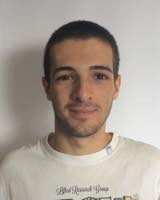
\includegraphics[height=0.8in]{PedroF} \\

\end{tabular}
\end{table}

\newpage
\tableofcontents
\newpage

\section{Introdução}
A primeira fase do projeto da UC Desenvolvimento de Sistemas de Software consistiu no desenvolvimento dos modelos de domínio, use cases e da interface com o utilizador para a aplicação ConfiguraFácil. 

Na segunda fase, desenvolvemos os diagramas de sequência, de pacotes, de implementação e de classes. Além disso, procedemos também a implementação da aplicação em si, utilizando os modelos desenhados previamente. Para tal, utilizamos DAOs para podermos fazer a conexão entre a base de dados e a aplicação em JAVA. Alterámos também alguns modelos que apresentamos na fase anterior, corrigindo para uma versão que mais se foca nos objetivos da aplicação que pretendíamos modelar.

A aplicação \textit{ConfiguraFácil} consiste numa ferramenta existente nos stands de automóveis, que permite junto dos clientes criar uma configuração para uma encomenda de um carro novo. A aplicação guia o cliente em cada fase da configuração, permitindo-lhe escolher componentes individuais ou pacotes pré-definidos. 

Da perspetiva do grupo, a aplicação apresenta os seguintes requisitos:
\begin{itemize}
	\item O cliente pode escolher a pintura, jantes e pneus, motorização e detalhes interiores e exteriores;
	\item O cliente pode também escolher um pacote pré-definido que consiste num agregado de componentes individuais;
	\item Cada componente deve ter uma designação, preço, lista de componentes incompatíveis e lista de componentes complementares;
	\item Sempre que um componente é adicionado à configuração, a aplicação deve verificar se existe alguma incompatibilidade com algum componente previamente selecionado. Se tal existir, o cliente pode optar por desistir da seleção feita ou remover o produto incompatível. Além disso, deve também verificar se é necessário instalar algum componente complementar. Caso aconteça, o cliente pode manter a opção e instalar os componentes necessários ou então desistir da seleção;
	\item Quando um pacote pré-definido é selecionado, devem ser feitas as verificações de dependência/incompatibilidade para cada um dos componentes do pacote;
	\item Deve haver descontos associados aos pacotes, ou seja, os pacotes devem ser mais baratos que a soma os preços individuais de cada um dos seus componentes;
	\item Se o cliente selecionar individualmente todos os componentes que compõem um pacote, a aplicação deve reconhecer tal pacote e aplicar o respetivo desconto;
	\item Após as escolhas básicas, como a pintura e a motorização, o cliente deve poder indicar um orçamento para a encomenda e o sistema deve propor a melhor configuração possível dentro do orçamento apresentado. Ou seja, a aplicação deve conseguir gerar uma configuração ótima dado um orçamento;
	\item Cada componente deve ter um stock associado;
	\item Sempre que chega um novo stock de componentes, o sistema deve conseguir determinar quais são os carros que podem ser produzidos;
	\item Os carros são produzidos por ordem de chegada à fila de configurações efetuadas pelos clientes.
\end{itemize}
Desta forma, procuramos cobrir todos estes requisitos, de forma a que a aplicação seja o mais completa e coesa possível. Além do referido, incluimos também as funcionalidades de registar, identificar, consultar e alterar clientes, login de funcionários (sendo que o administrador pode registar, remover ou alterar os dados destes) e as funcionalidades relativas à gestão de fábrica de encomendar stock e registar a sua entrada no sistema.

\begin{center}
\section*{1ª Fase}
\end{center}

\section{Diagrama de Domínio}
Para a aplicação que nos foi proposta e que descrevemos acima, desenvolvemos o diagrama de domínio que apresentamos de seguida:
\begin{center}
 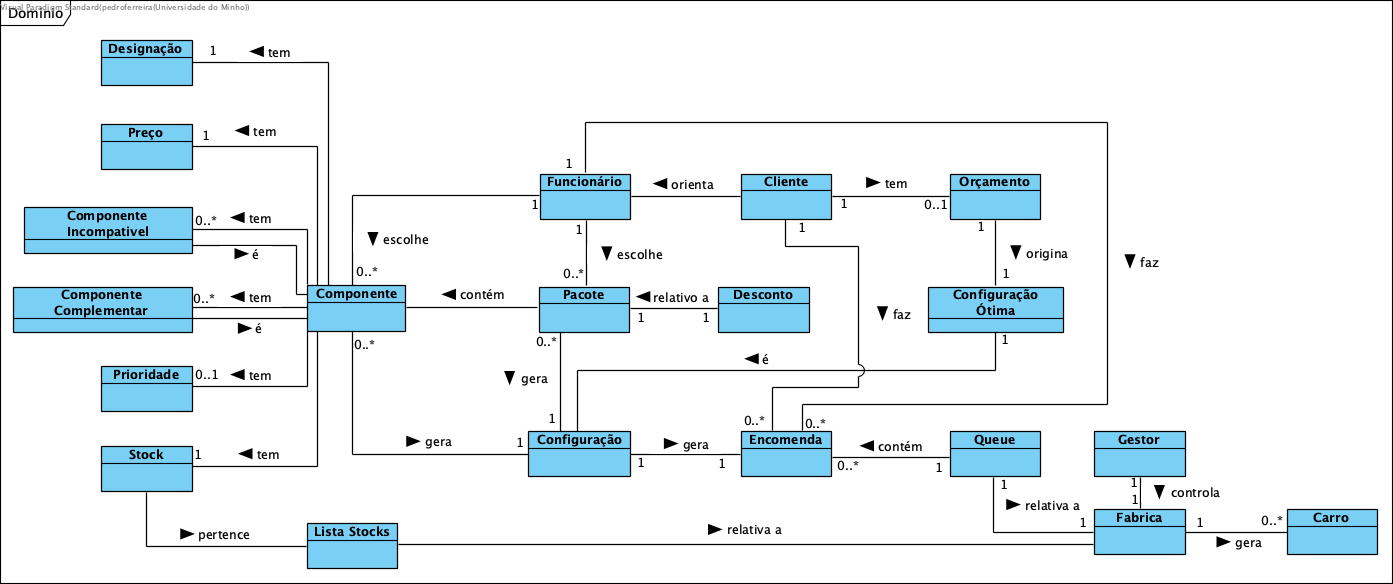
\includegraphics[width = 6.5in]{Dominio.png}
\end{center}

\newpage
\section{Diagrama de Use Cases}
\label{useCases}
Os Use Cases por nós apresentados e especificados na secção seguinte foram organizados em seis diagramas:
\begin{enumerate}
	\item Geral
		\begin{center}
 			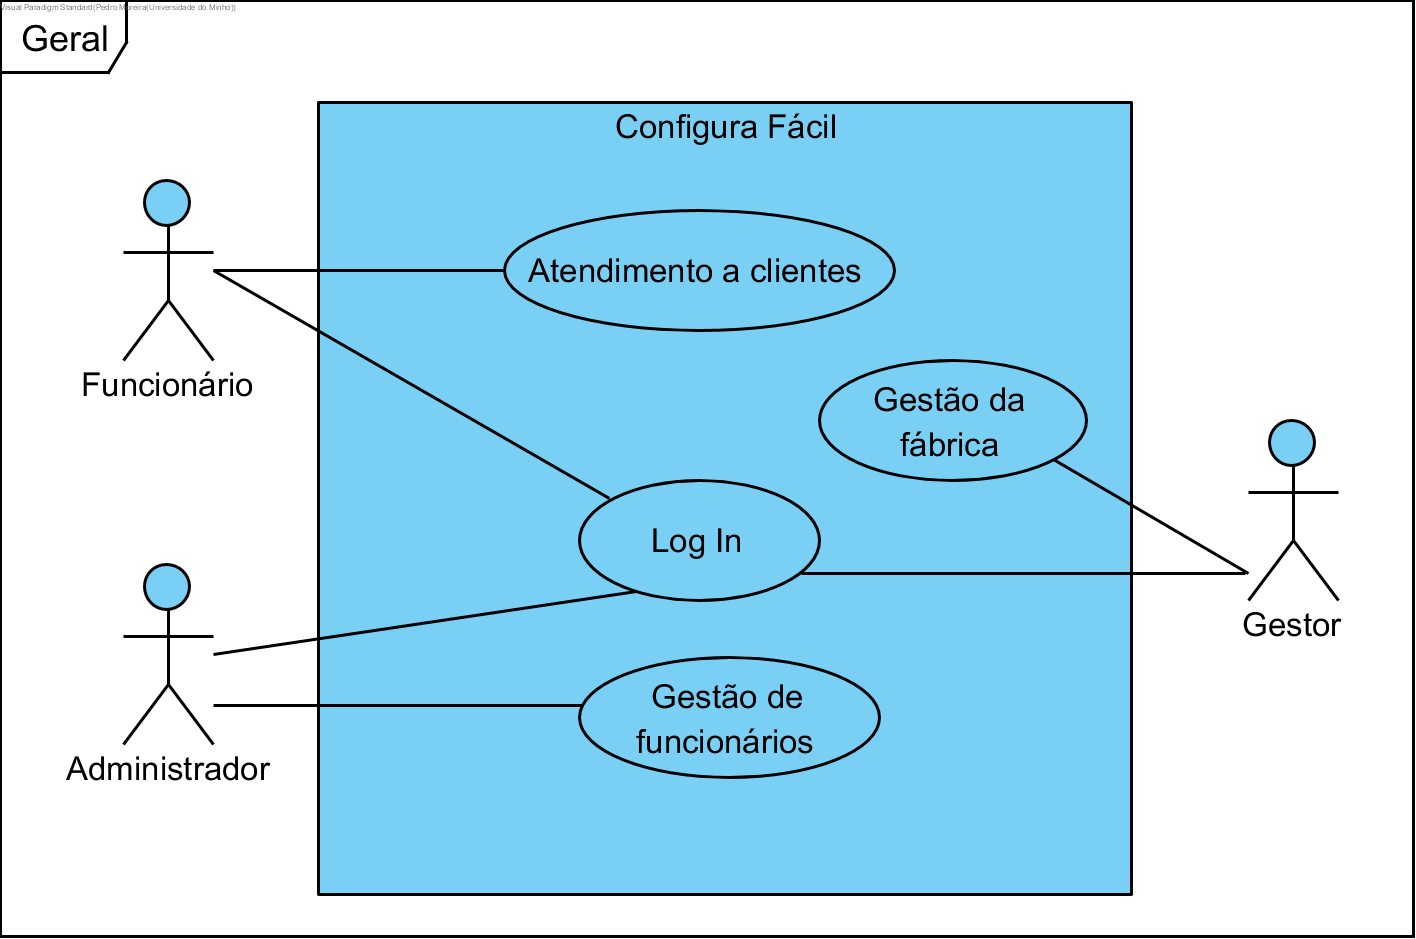
\includegraphics[]{Geral.png}
		\end{center}
	\item Gestão de Funcionários
		\begin{center}
 			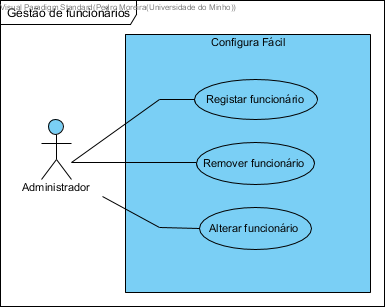
\includegraphics[]{Gestao_de_funcionarios.png}
		\end{center}\newpage
	\item Gestão de Clientes
		\begin{center}
 			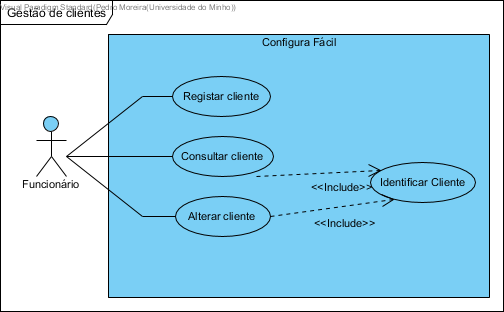
\includegraphics[]{Gestao_de_clientes.png}
		\end{center}
	\item Atendimento a Clientes
		\begin{center}
 			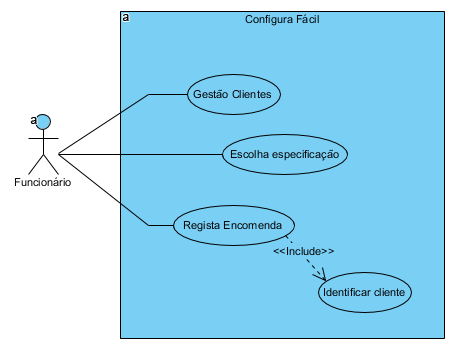
\includegraphics[]{Atendimento_a_clientes.png}
		\end{center}\newpage
	\item Escolha da Especificação
		\begin{center}
 			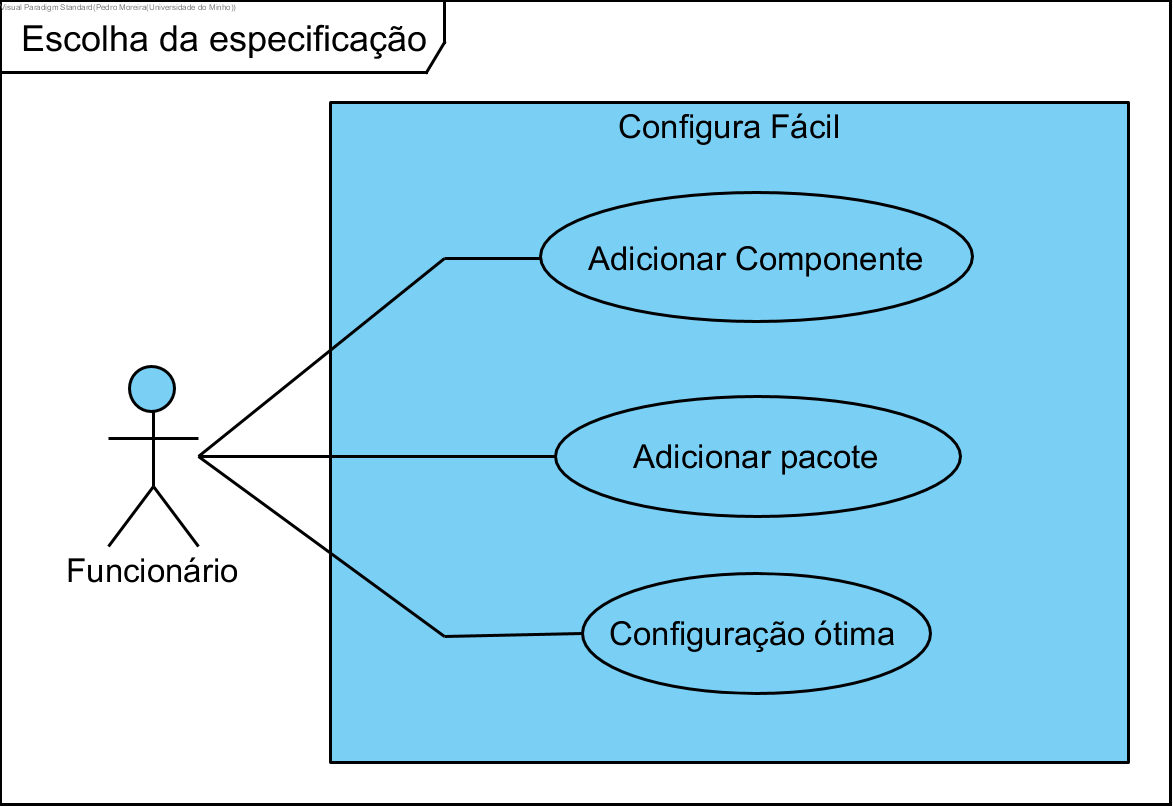
\includegraphics[]{Escolha_da_especificacao.png}
		\end{center}
	\item Gestão da Fábrica
		\begin{center}
 			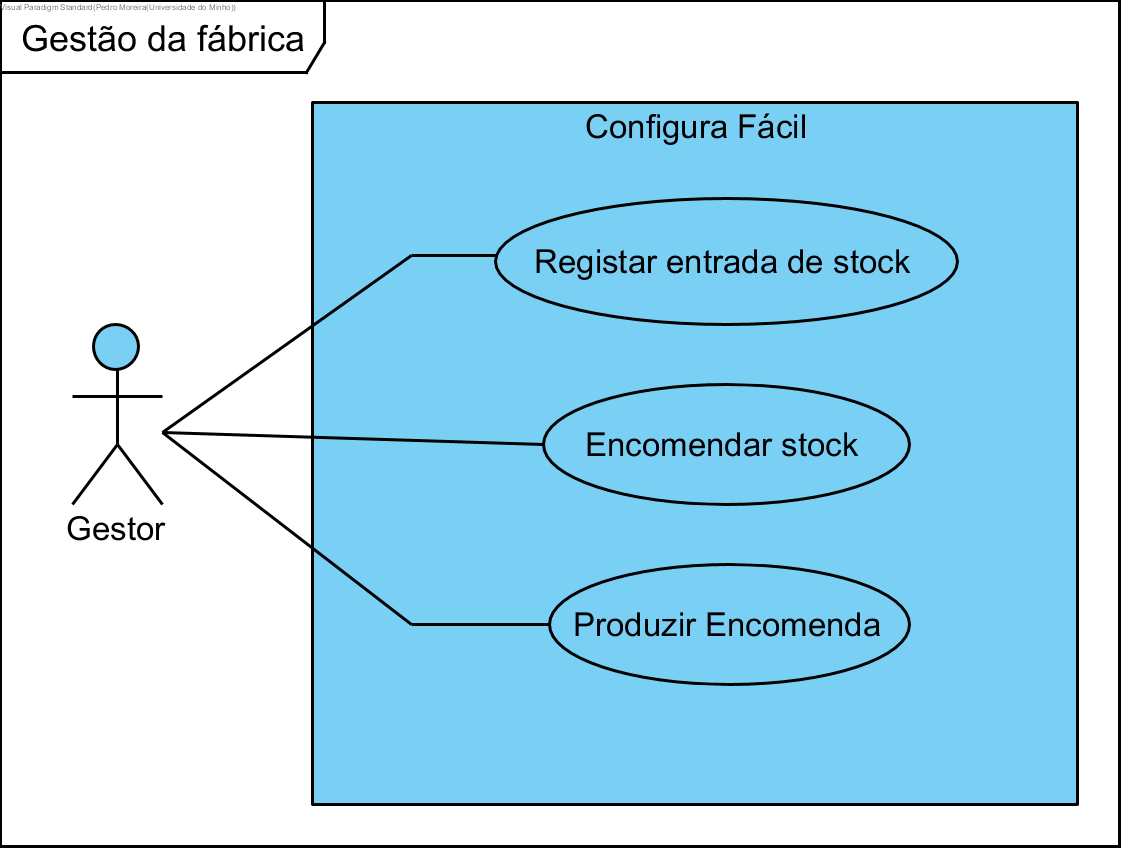
\includegraphics[]{Gestao_da_fabrica.png}
		\end{center}
\end{enumerate}

\newpage
\section{Especificação de Use Cases}
Nesta secção vamos expor as tabelas de especificação que fizemos para cada um dos Use Cases presentes nos diagramas da secção \ref{useCases}.

Para melhor organização, decidimos dividir as tabelas em Excel da especificação dos Use Cases em quatro ficheiros: 
\begin{enumerate}
	\item Login

 		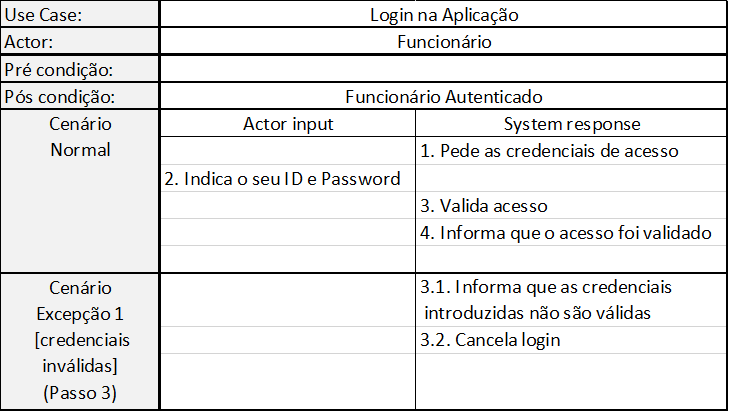
\includegraphics[width = 5in]{login.png} \newpage
	\item  Atendimento a Clientes
	\begin{center}
 		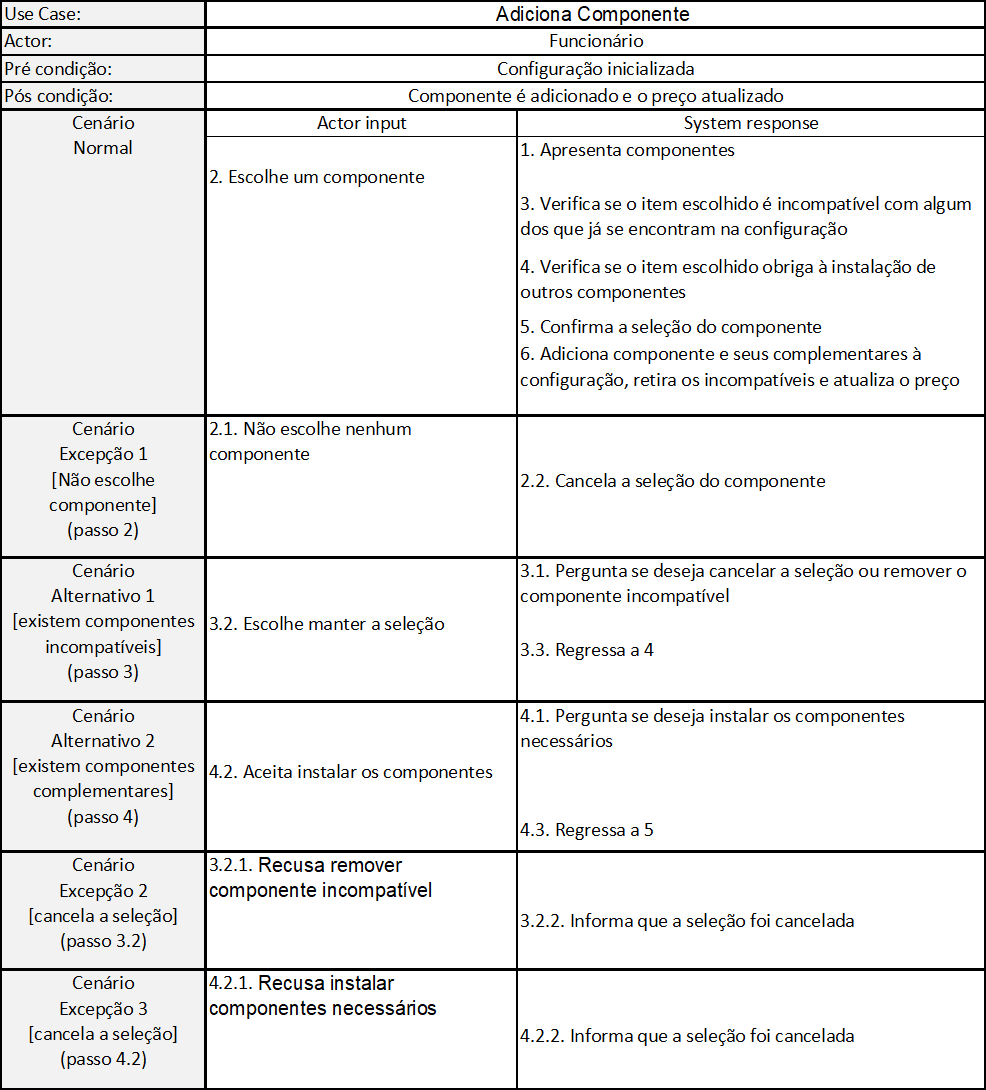
\includegraphics[width = 5in]{ac_adicionacomp.png} 
 		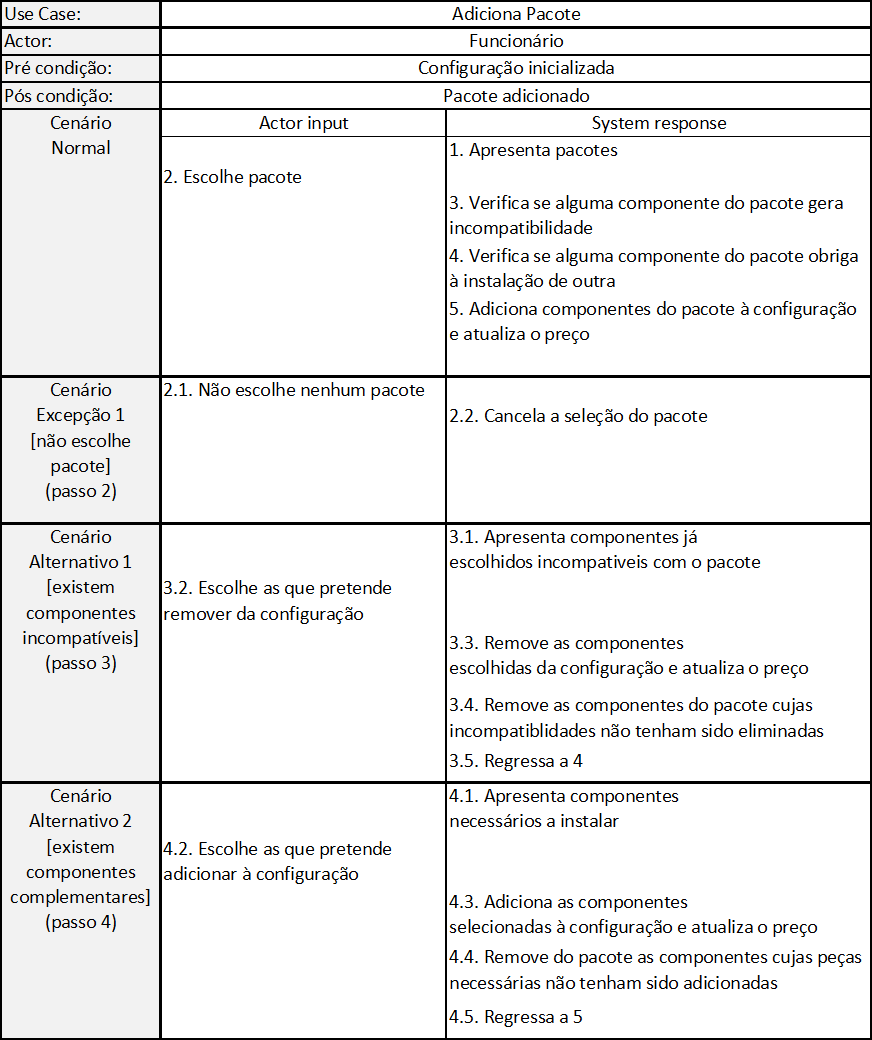
\includegraphics[width = 5in]{ac_adicionapacote.png} 
		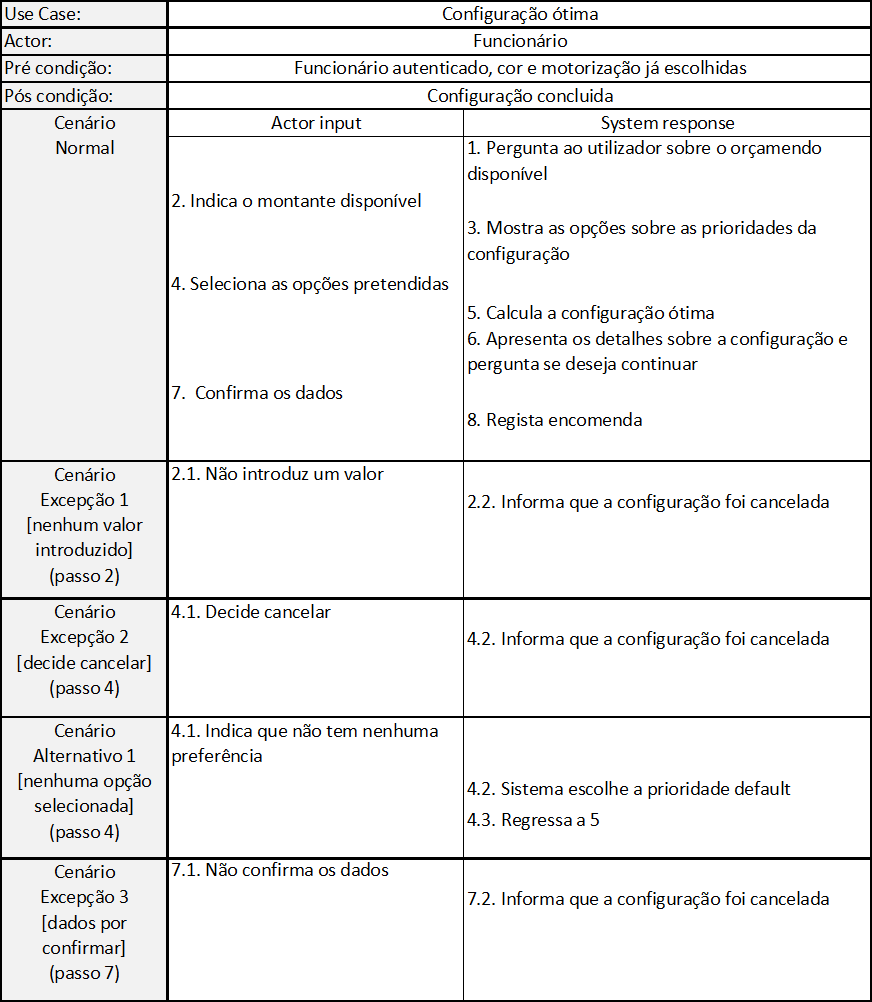
\includegraphics[width = 5in]{ac_configotima.png}
	\end{center}
	\begin{center}
		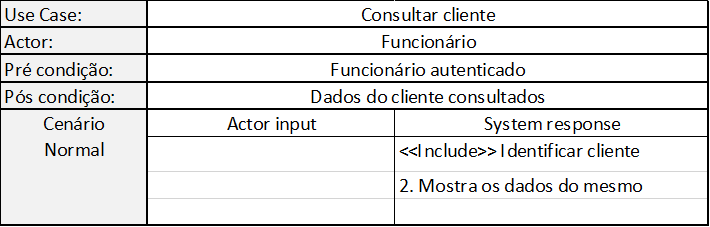
\includegraphics[width = 5in]{ac_consultarcliente.png} 
	\end{center}
	\begin{center}
		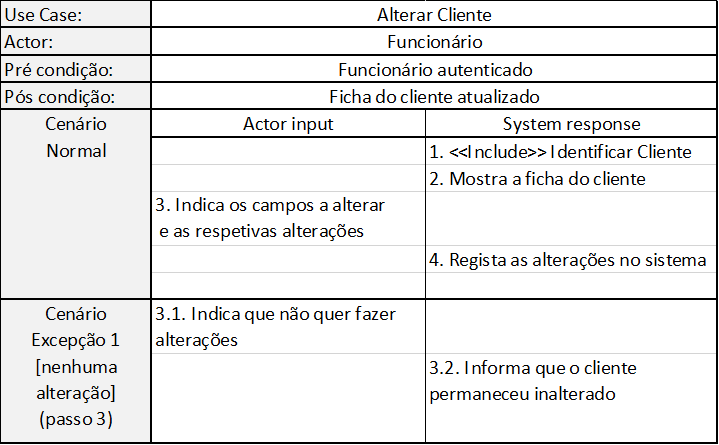
\includegraphics[width = 5in]{ac_altcliente.png}
	\end{center}
	\begin{center}
		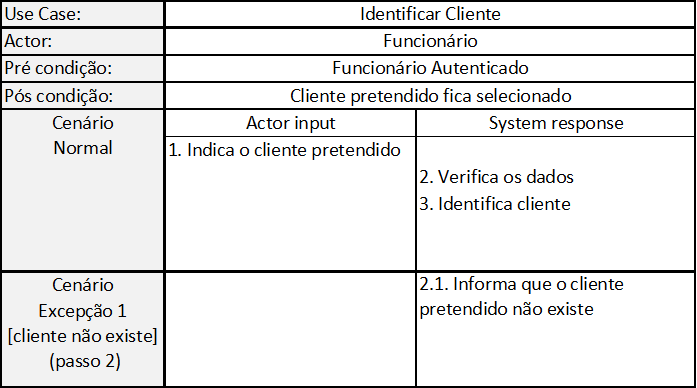
\includegraphics[width = 5in]{ac_idcliente.png}
	\end{center}
	\begin{center}
		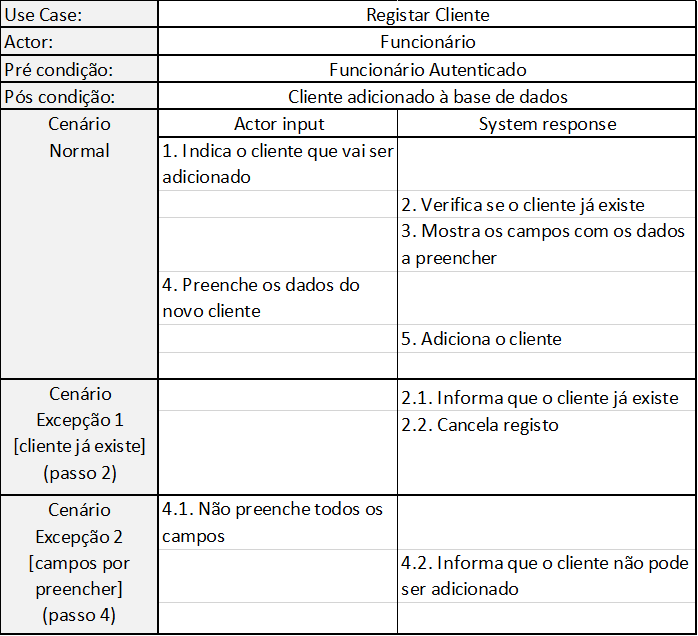
\includegraphics[width = 5in]{ac_regcliente.png}
	\end{center}
	\begin{center}
		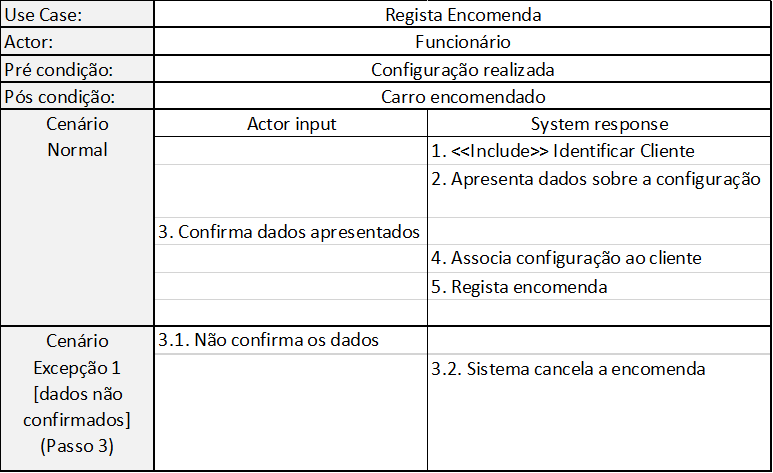
\includegraphics[width = 5in]{ac_regenc.png}
	\end{center}
	\newpage
	\item Gestão de Fábrica
	\begin{center}
		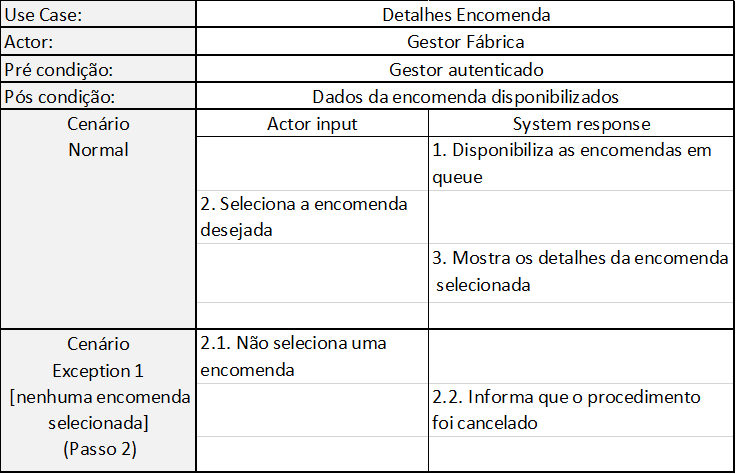
\includegraphics[width = 5in]{gf_consultarencomenda.png} 
	\end{center}
	\begin{center}
 		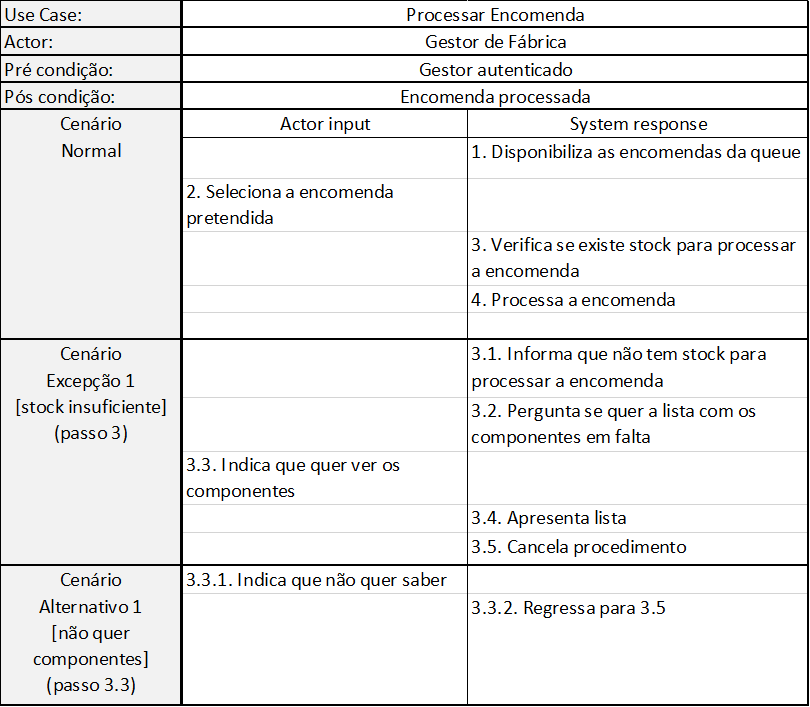
\includegraphics[width = 5in]{gf_processarencomenda.png} 
		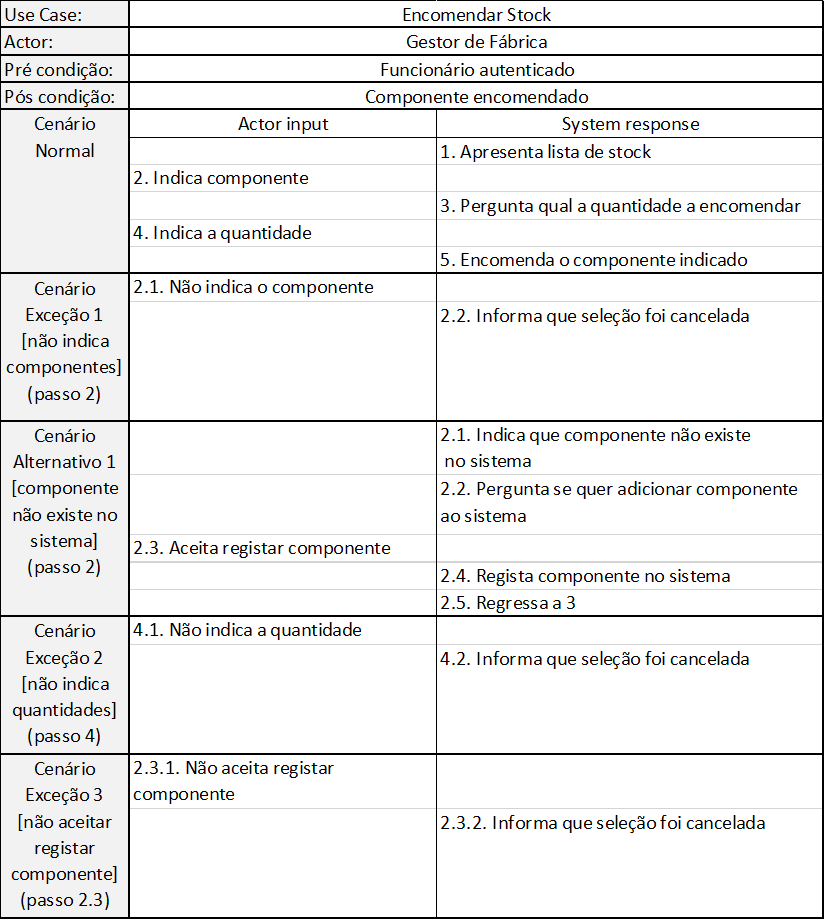
\includegraphics[width = 5in]{gf_encomendarstock.png} 
		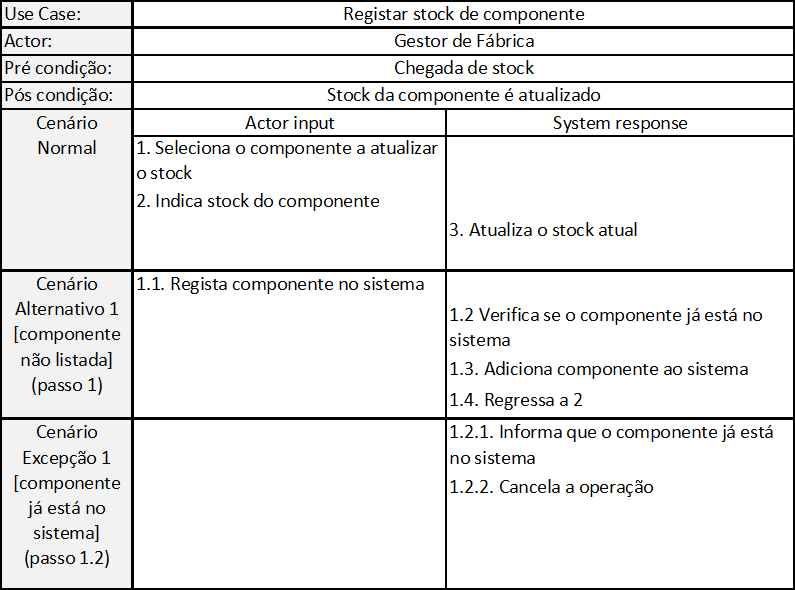
\includegraphics[width = 5in]{gf_registarstock.png}
	\end{center}
	\newpage
	\item Gestão de Funcionários
	\begin{center}
		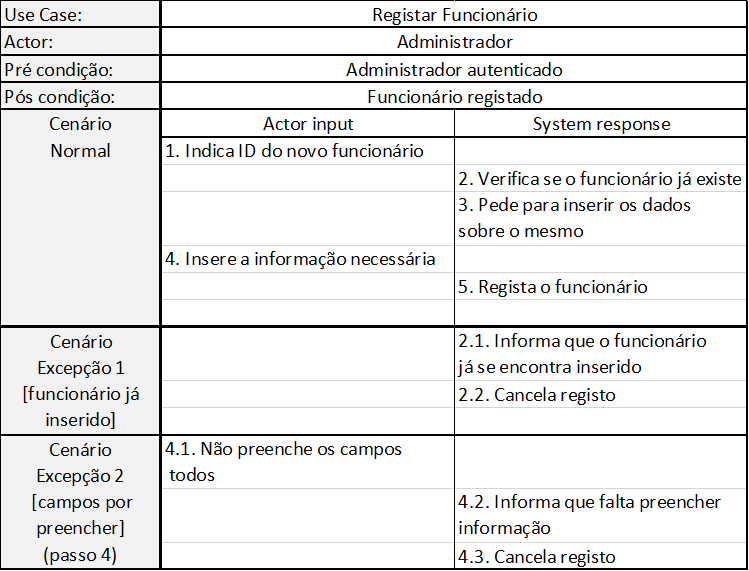
\includegraphics[width = 5in]{gfunc_registar.png} 
	\end{center}
	\begin{center}
 		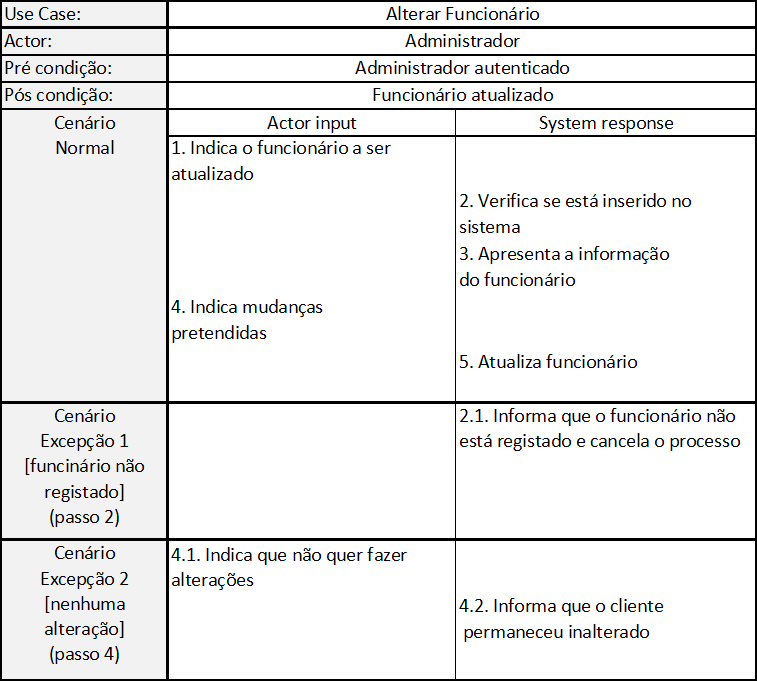
\includegraphics[width = 5in]{gfunc_alterar.png} 
	\end{center}
	\begin{center}
		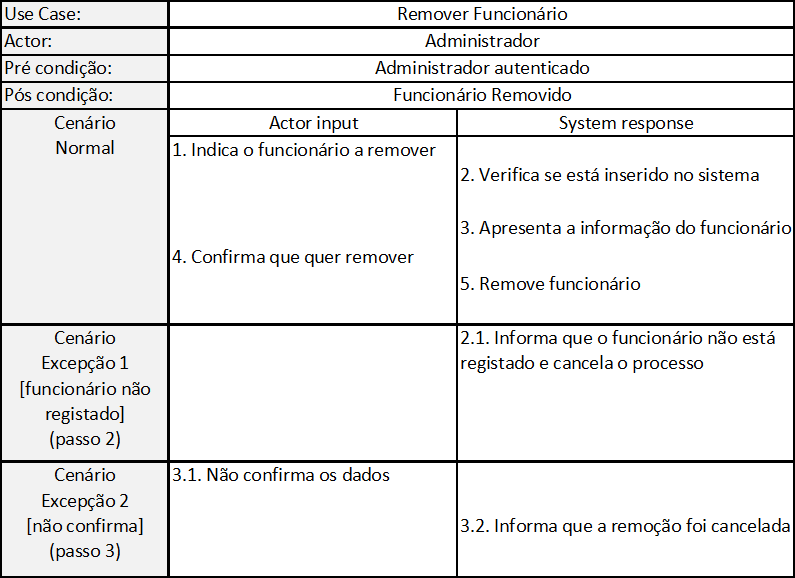
\includegraphics[width = 5in]{gfunc_remover.png}
	\end{center}
\end{enumerate}

\section{Protótipo de Interface}
O protótipo de interface para a aplicação foi feito com o \textit{Pencil}, ferramenta aconselhada pelos docentes da UC.

A página inicial do programa é a pagina de login.
\begin{center}
 	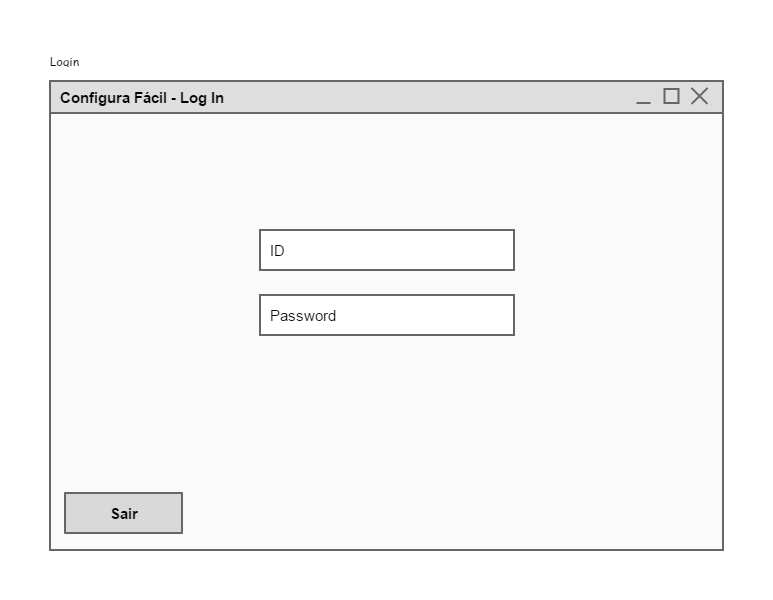
\includegraphics[width = 5in]{configura_fcil_root.png}
\end{center}

Daqui, o utilizador pode ir para uma das seguintes janelas, dependendo do seu estatuto na aplicação:

\begin{center}
 	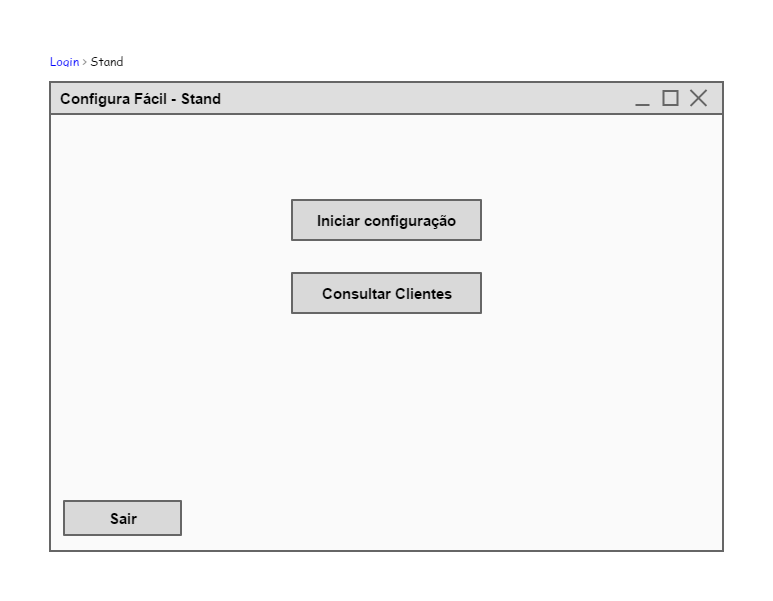
\includegraphics[width = 5.5in]{configura_fcil_stand.png}

 	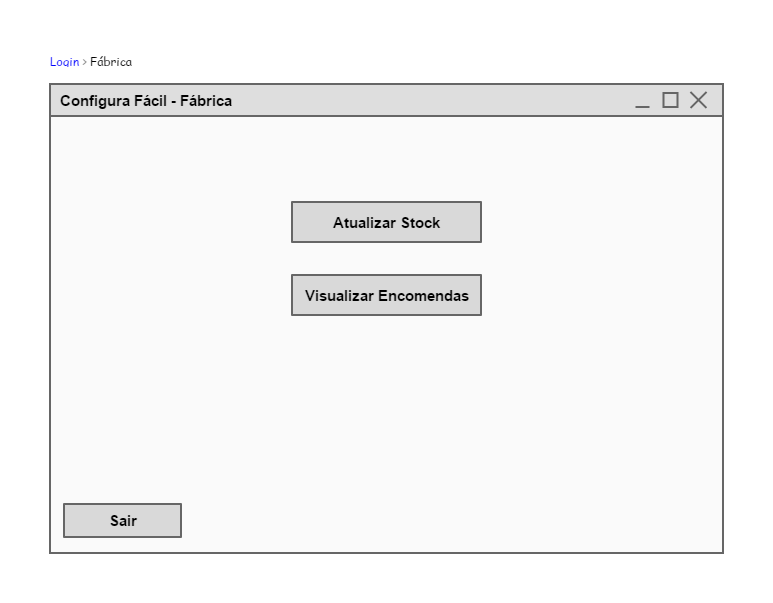
\includegraphics[width = 5.5in]{configura_fcil_fbrica.png}

 	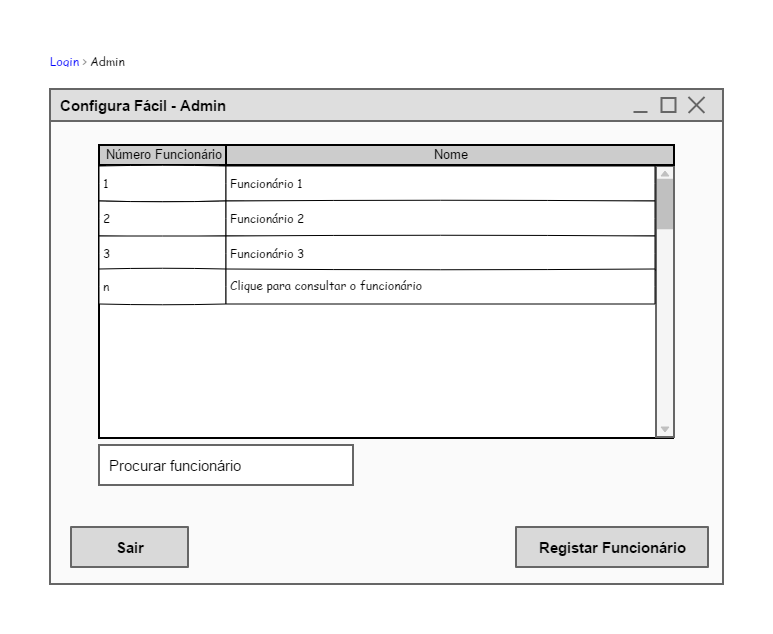
\includegraphics[width = 5.5in]{configura_fcil_admin.png}
\end{center}


A partir da janela do Stand encontramos a seguinte interface:
\begin{center}
 	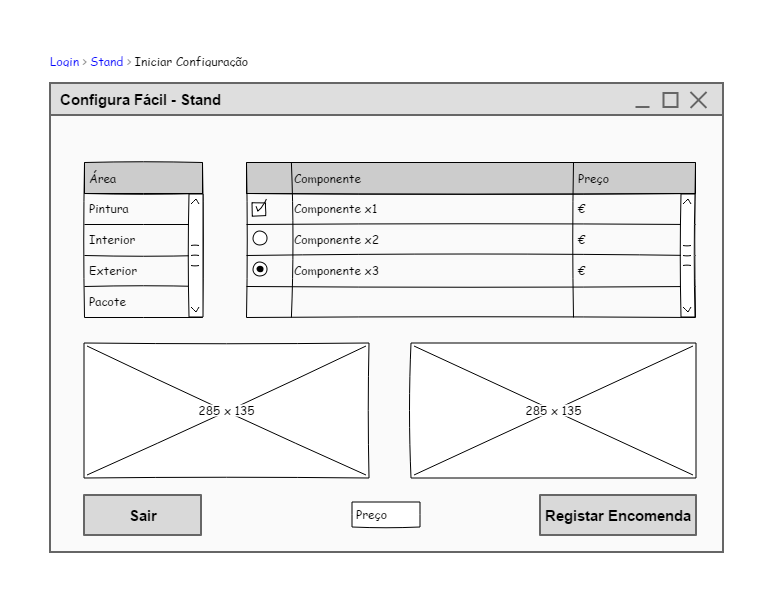
\includegraphics[width = 5in]{configurao_de_carro.png}

 	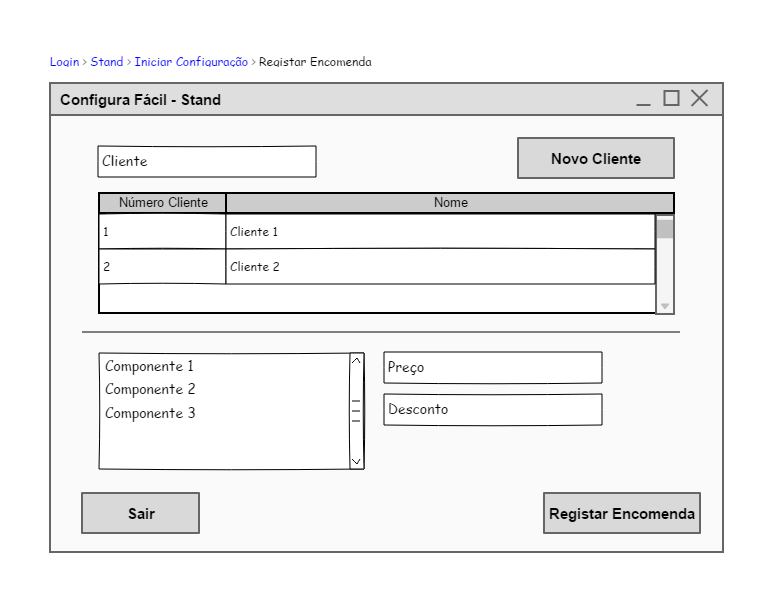
\includegraphics[width = 5.5in]{registar_encomenda.png}

 	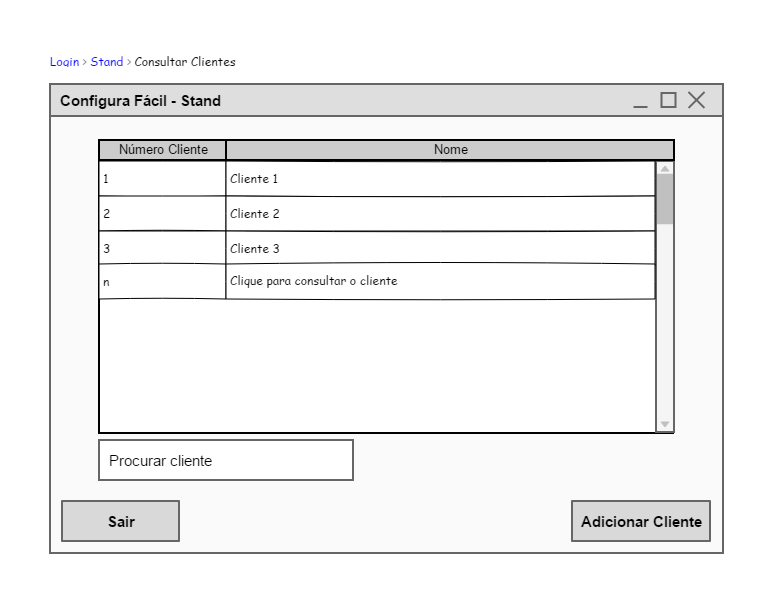
\includegraphics[width = 5.5in]{consultar_clientes.png}
	
	\begin{table}[]
		\begin{tabular}{cc}
 			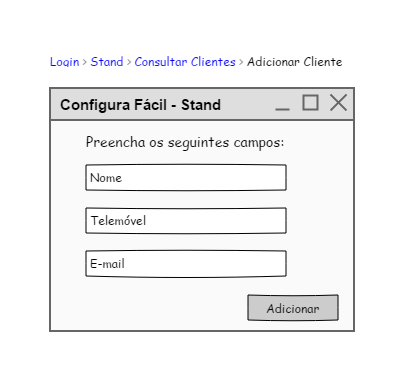
\includegraphics[width = 3in]{adicionar_cliente.png}	& 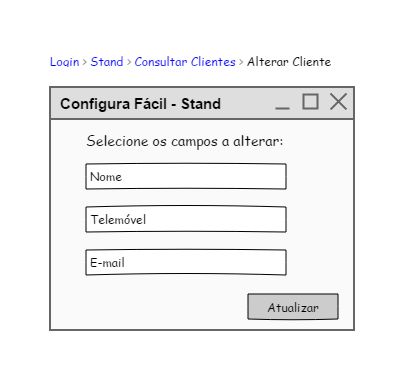
\includegraphics[width = 3in]{alterar_cliente.png}
		\end{tabular}
	\end{table}
 	 	
\end{center}

Já quando o utilizador é um gestor da fábrica, a interface gráfica que o guiará pela aplicação é a seguinte:
\begin{center}
	\begin{table}[!htbp]
		\begin{tabular}{cc}
 			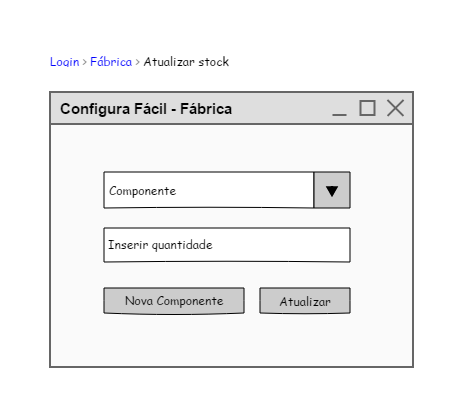
\includegraphics[width = 3in]{atualizar_stock.png} & 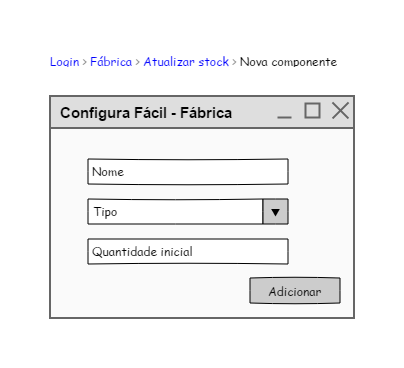
\includegraphics[width = 3in]{nova_componente.png}
		\end{tabular}
	\end{table}

 	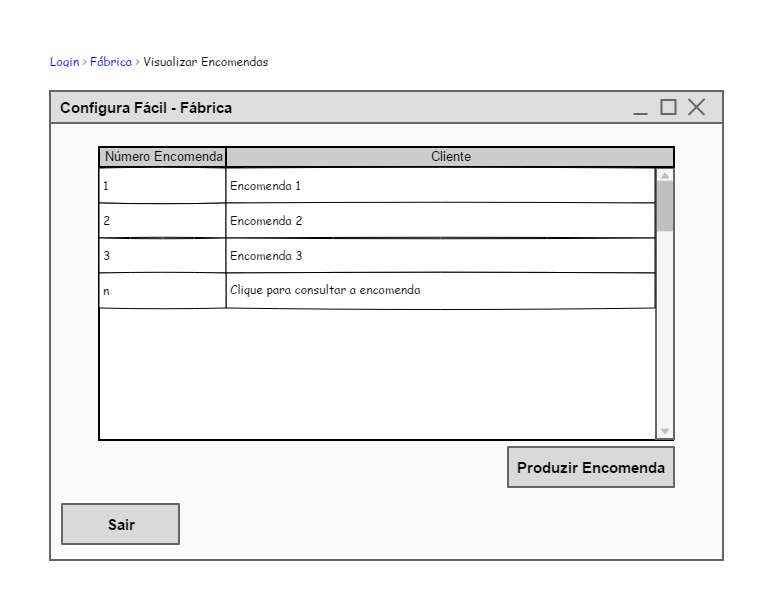
\includegraphics[width = 5.5in]{visualizar_encomendas.png}

\end{center}

Por fim, quando o funcionário faz o Login como Admistrador será esta a sua visão da aplicação:
\begin{center}
	\begin{table}[!htbp]
		\begin{tabular}{cc}
 			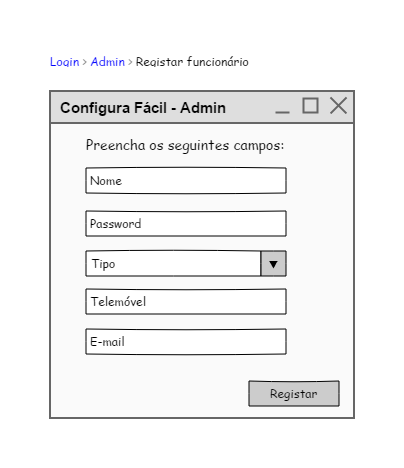
\includegraphics[width = 3in]{registar_funcionrio.png} & 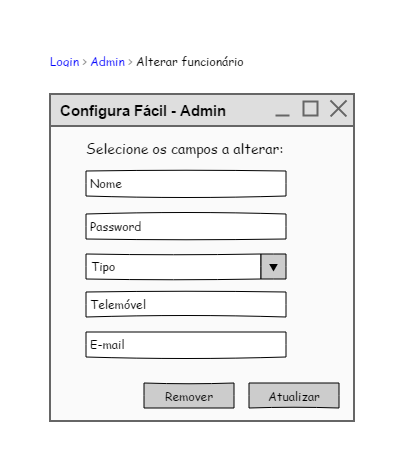
\includegraphics[width = 3in]{alterar_funcionrio.png}
		\end{tabular}
	\end{table}

\end{center}


\section{Diagrama de Máquinas de Estado}
O diagrama de Máquinas de Estado relativo à interface do programa é o seguinte:
	\begin{center}
		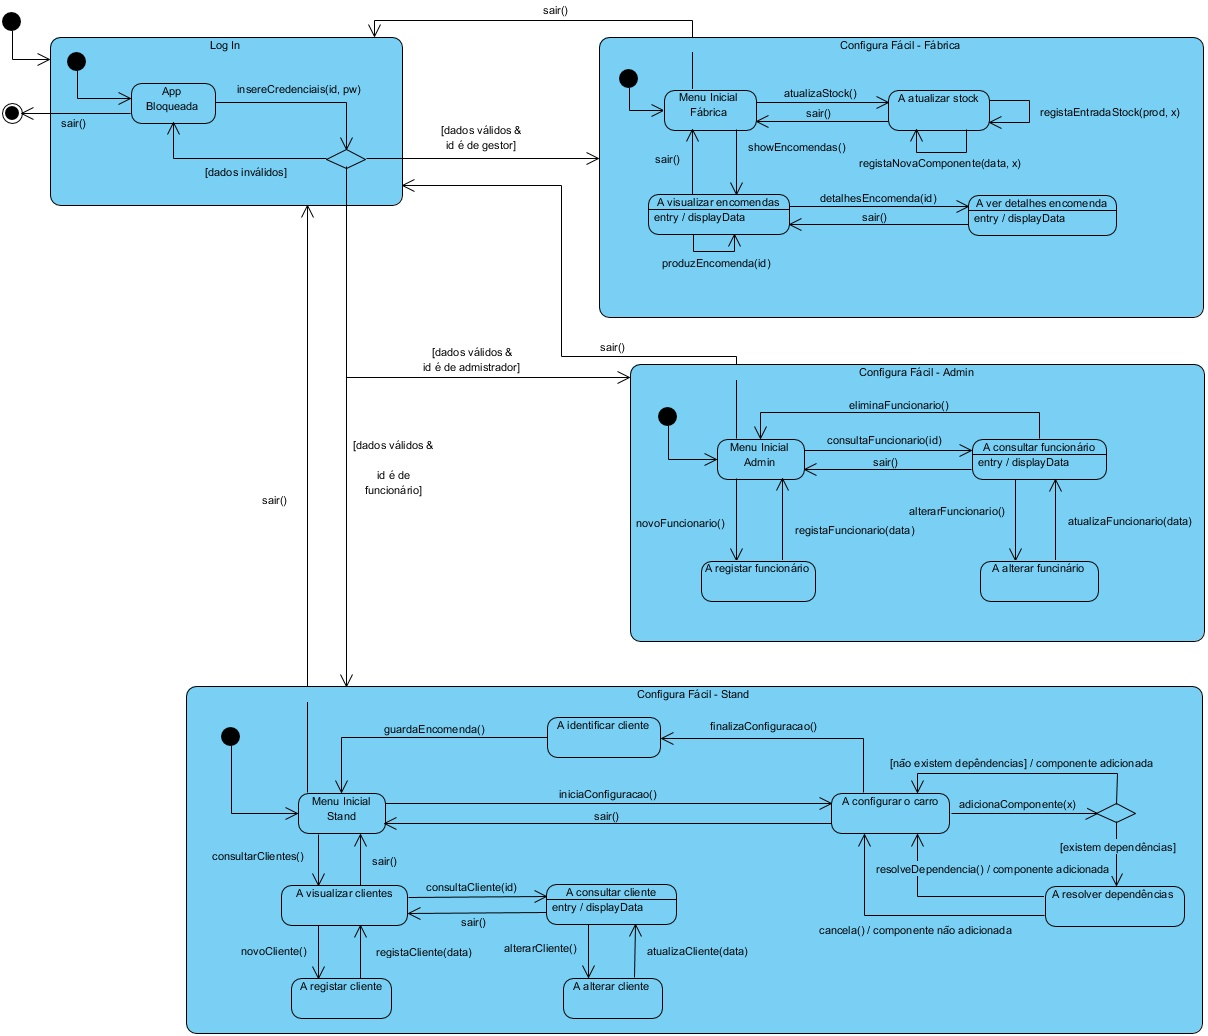
\includegraphics[width = 6in]{Maquina_de_Estado.jpg}
	\end{center}
	
\newpage

\begin{center}
\section*{2ª Fase}
\end{center}

\section{Diagramas de Sequência}
A segunda fase do projeto principiou com a modelação dos diagramas de sequência, partindo da especificação dos Use Cases feita na fase anterior. Assim sendo, temos os seguintes diagramas:

\begin{enumerate}
	\item Adiciona Componente
		\begin{center}
 			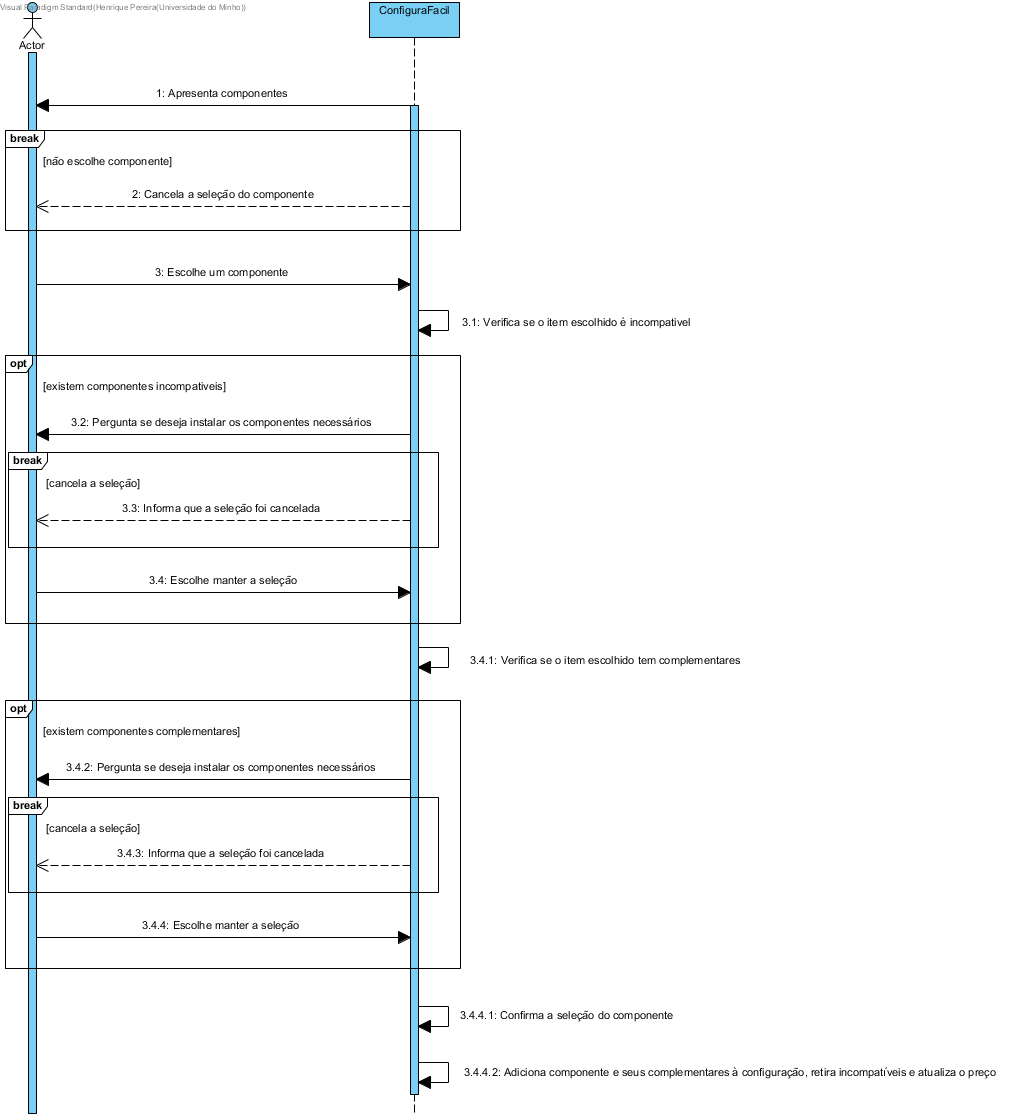
\includegraphics[width = 6in]{dss_adiciona_componente.png}
		\end{center}
	\item Adiciona Pacote
		\begin{center}
 			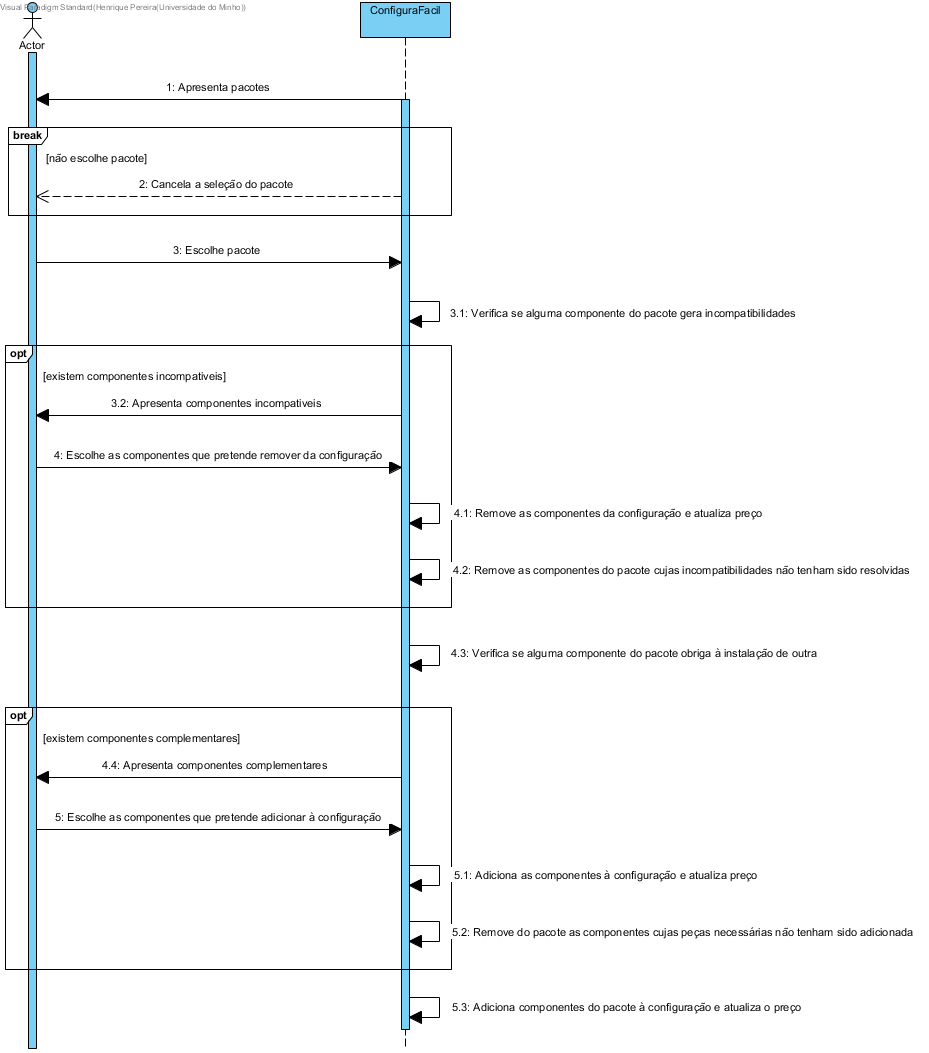
\includegraphics[width = 6in]{dss_adiciona_pacote.png}
		\end{center}\newpage
	\item Alterar Cliente
		\begin{center}
 			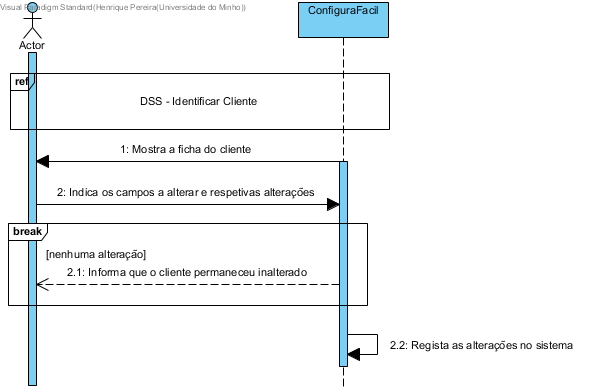
\includegraphics[width = 6in]{dss_alterar_cliente.png}
		\end{center}
	\item Alterar Funcionário
		\begin{center}
 			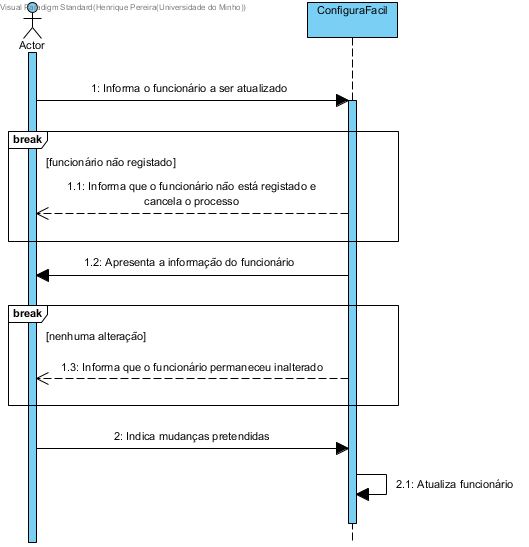
\includegraphics[width = 6in]{dss_alterar_funcionario.png}
		\end{center}\newpage
	\item Configuração Ótima
		\begin{center}
 			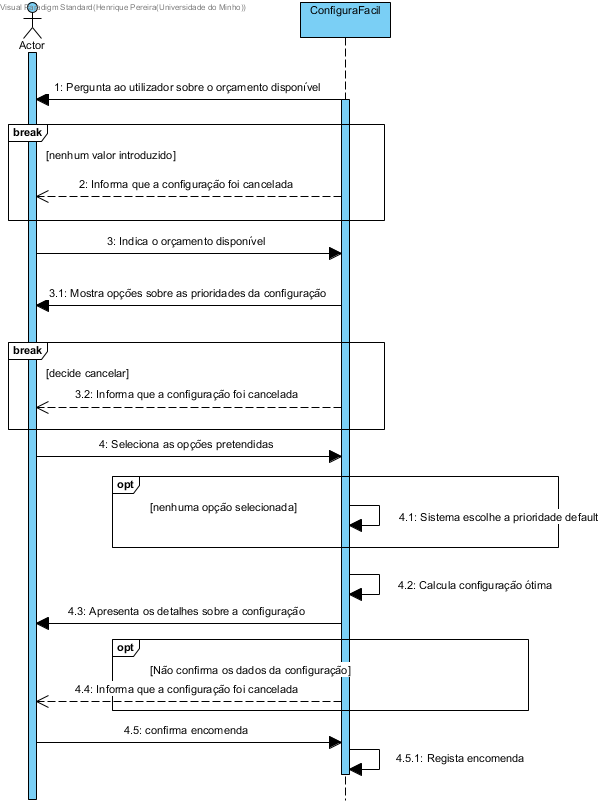
\includegraphics[width = 6in]{dss_configuracao_otima.png}
		\end{center}
	\item Consultar Cliente
		\begin{center}
 			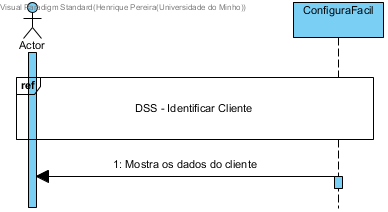
\includegraphics[width = 6in]{dss_consultar_cliente.png}
		\end{center}
	\item Consultar Encomenda
		\begin{center}
 			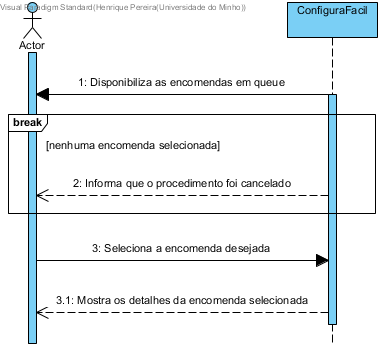
\includegraphics[width = 6in]{dss_consultar_encomenda.png}
		\end{center}
	\item Encomendar Stock
		\begin{center}
 			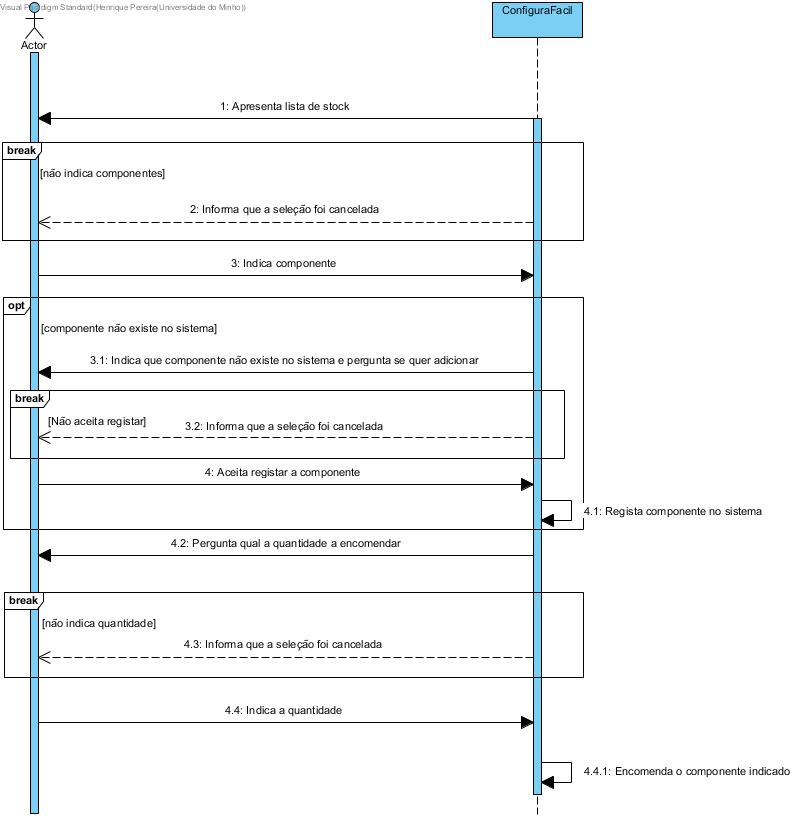
\includegraphics[width = 6in]{dss_encomendar_stock.png}
		\end{center}
	\item Identificar Cliente
		\begin{center}
 			\includegraphics[width = 6in]{dss_identificar_cliente.png}
		\end{center}
	\item Login
		\begin{center}
 			\includegraphics[width = 6in]{dss_login.png}
		\end{center}
	\item Processa Encomenda
		\begin{center}
 			\includegraphics[width = 6in]{dss_processa_encomenda.png}
		\end{center}
	\item Registar Cliente
		\begin{center}
 			\includegraphics[width = 6in]{dss_registar_cliente.png}
		\end{center}
	\item Registar Encomenda
		\begin{center}
 			\includegraphics[width = 6in]{dss_registar_encomenda.png}
		\end{center}
	\item Registar Funcionário
		\begin{center}
 			\includegraphics[width = 6in]{dss_registar_funcionario.png}
		\end{center}
	\item Registar Stock de Componente
		\begin{center}
 			\includegraphics[width = 6in]{dss_registar_stock.png}
		\end{center}
	\item Remover Funcionário
		\begin{center}
 			\includegraphics[width = 6in]{dss_remover_funcionario.png}
		\end{center}
\end{enumerate}

\section{Diagrama de Pacotes}
De forma a organizarmos melhor a aplicação, dividimos o sistema geral em quatro subsistemas: o Facade (que corresponde à ConfiguraFácil), o gContas, o gConfig e o gFabrica. Como tal, construímos o seguinte diagrama de pacotes:
\begin{center}
 	\includegraphics[width=6in]{pacotes.jpg}
\end{center}

\section{Diagramas de Sequência de Subsistema}
O passo seguinte foi, partindo dos diagramas de sequência e conhecendo agora os subsistemas existentes, modelar os diagramas de sequência de subsistema, para depois podemos proseguir com os diagramas de implementação.

Ora, temos então o seguinte:
\begin{enumerate}
	\item Adiciona Componente
		\begin{center}
 			\includegraphics[width = 6in]{dsss_adiciona_componente.png}
		\end{center}
	\item Adiciona Pacote
		\begin{center}
 			\includegraphics[width = 6in]{dsss_adiciona_pacote.png}
		\end{center}\newpage
	\item Alterar Cliente
		\begin{center}
 			\includegraphics[width = 6in]{dsss_alterar_cliente.png}
		\end{center}
	\item Alterar Funcionário
		\begin{center}
 			\includegraphics[width = 6in]{dsss_alterar_funcionario.png}
		\end{center}\newpage
	\item Configuração Ótima
		\begin{center}
 			\includegraphics[width = 6in]{dsss_configuracao_otima.png}
		\end{center}
	\item Consultar Cliente
		\begin{center}
 			\includegraphics[width = 6in]{dsss_consultar_cliente.png}
		\end{center}
	\item Consultar Encomenda
		\begin{center}
 			\includegraphics[width = 6in]{dsss_consultar_encomenda.png}
		\end{center}
	\item Encomendar Stock
		\begin{center}
 			\includegraphics[width = 6in]{dsss_encomendar_stock.png}
		\end{center}
	\item Identificar Cliente
		\begin{center}
 			\includegraphics[width = 6in]{dsss_identificar_cliente.png}
		\end{center}
	\item Login
		\begin{center}
 			\includegraphics[width = 6in]{dsss_login.png}
		\end{center}
	\item Processa Encomenda
		\begin{center}
 			\includegraphics[width = 6in]{dsss_processa_encomenda.png}
		\end{center}
	\item Registar Cliente
		\begin{center}
 			\includegraphics[width = 6in]{dsss_registar_cliente.png}
		\end{center}
	\item Registar Encomenda
		\begin{center}
 			\includegraphics[width = 6in]{dsss_registar_encomenda.png}
		\end{center}
	\item Registar Funcionário
		\begin{center}
 			\includegraphics[width = 6in]{dsss_registar_funcionario.png}
		\end{center}
	\item Registar Stock de Componente
		\begin{center}
 			\includegraphics[width = 6in]{dsss_registar_stock.png}
		\end{center}
	\item Remover Funcionário
		\begin{center}
 			\includegraphics[width = 6in]{dsss_remover_funcionario.png}
		\end{center}
\end{enumerate}

\section{Diagramas de Sequência de Implementação}
Como foi referido, podemos agora desenhar os diagramas de sequência de implementação. Com estes já definidos, podemos começar a escrever o código para a aplicação, partindo de uma base bastante consistente.

Para tal, modelamos os ditos diagramas da seguinte maneira:
\begin{enumerate}
	\item Adiciona Componente
		\begin{center}
 			\includegraphics[]{dsi_adiciona_componente.png}
		\end{center}
	\item Adiciona Pacote
		\begin{center}
 			\includegraphics[]{dsi_adiciona_pacote.png}
		\end{center}\newpage
	\item Alterar Cliente
		\begin{center}
 			\includegraphics[]{dsi_alterar_cliente.png}
		\end{center}
	\item Alterar Funcionário
		\begin{center}
 			\includegraphics[]{dsi_alterar_funcionario.png}
		\end{center}\newpage
	\item Configuração Ótima
		\begin{center}
 			\includegraphics[]{dsi_configuracao_otima.png}
		\end{center}
	\item Consultar Cliente
		\begin{center}
 			\includegraphics[]{dsi_consultar_cliente.png}
		\end{center}
	\item Consultar Encomenda
		\begin{center}
 			\includegraphics[]{dsi_consultar_encomenda.png}
		\end{center}
	\item Encomendar Stock
		\begin{center}
 			\includegraphics[]{dsi_encomendar_stock.png}
		\end{center}
	\item Identificar Cliente
		\begin{center}
 			\includegraphics[]{dsi_identificar_cliente.png}
		\end{center}
	\item Login
		\begin{center}
 			\includegraphics[]{dsi_login.png}
		\end{center}
	\item Processa Encomenda
		\begin{center}
 			\includegraphics[]{dsi_processa_encomenda.png}
		\end{center}
	\item Registar Cliente
		\begin{center}
 			\includegraphics[]{dsi_registar_cliente.png}
		\end{center}
	\item Registar Encomenda
		\begin{center}
 			\includegraphics[]{dsi_registar_encomenda.png}
		\end{center}
	\item Registar Funcionário
		\begin{center}
 			\includegraphics[]{dsi_registar_funcionario.png}
		\end{center}
	\item Registar Stock de Componente
		\begin{center}
 			\includegraphics[]{dsi_registar_stock.png}
		\end{center}
	\item Remover Funcionário
		\begin{center}
 			\includegraphics[]{dsi_remover_funcionario.png}
		\end{center}
\end{enumerate}

\section{Diagrama de Classes}
Partindo do Modelo de Domínio e dos diagramas de sequência de implementação, podemos definir o Diagrama de Classes:
\begin{center}
 	\includegraphics[width=6in]{Classes.png}
\end{center}

\section{DAOs}

\section{Implementação}


\section{Análise Crítica}
Nesta primeira fase do trabalho pediram-nos para fazer uma análise mais abstrata de modo a criar uma primeira imagem e ideia sobre a aplicação que estamos a desenvolver. A nossa abordagem começou pelo desenvolvimento do modelo domínio. Aqui tentamos estabelecer as principais entidades e as relações entre as mesmas de modo a criar a nossa primeira interpretação sobre o problema. Inicialmente, deparamo-nos com alguns erros de interpretação do enunciado como a função do cliente na aplicação que inicialmente achavamos que ia ser o principal utilizador e mais tarde foi alterado. Esta parte da modulação fez como que a nossa visão sobre o que queriamos para a aplicação ficasse mais clara e expressa de uma forma mais simplista. Ao modelo de domínio seguiu-se o desenvolvimento dos Use Case. Quando começamos o desenvolvimento dos mesmos, focamo-nos essencialmente em descrever a ação entre os atores e a aplicação. Esta descrição foi demasiado detalhada, fornecia informação que não era precisa e sobretudo limitava muito aquilo que queriamos fazer da aplicação. Como ainda nos encontravamos numa fase inicial decidimos refletir melhor sobre a nossa solução e chegamos à conclusão que eram limitações que não queriamos ter. A isto seguiu-se uma restruturação do problema de uma forma máis genérica que descrevia, na mesma, todas as funcionalidades dando-nos uma margem maior para aquilo que pode vir a ser a nossa aplicação.
Seguidamente demos inicio ao desenvolvimento das máquinas de estado. Aqui tentamos recriar os diversos estados da nossa aplicação e entender como é que estes alternavam entre si. O nosso principal obstáculo foi a dificuldade em exprimir os estados durante a personalização de uma configuração, no entanto após ter sido ultrapassada facilitou a forma como iriamos desenvolver o prótotipo da interface gráfica e levou-nos a uma melhor compreensão sobre a implementação das diversas funcionalidades. Por fim, chegou a altura de desenhar o primeiro prótotipo. Focamo-nos essencialmente em conseguir arranjar maneiras de implementar todas as nossas funcionalidades que tinhamos previstas seguindo os nossos Use Cases. De um modo geral, esta modelação ajudou-nos a prever futuros problemas e contribuiu para conseguir formular aquilo que queremos para o futuro da aplicação.

\textcolor{red}{ANÁLISE CRÍTICA DA 2ª FASE}

\end{document}
